\section{Présentation du projet}

\paragraph{}
Nous avons proposé notre propre projet dans l’optique de créer un jeu pour téléphone mobile, de sa conception jusqu’à sa mise en ligne. Le concept de base est de créer un “jeu de rythme”, à l'aide du moteur de jeu Unity. Nous nomerons notre jeu \textbf{Heliko} (Escargot en Esperanto).

\paragraph{}
La difficulté reléve dans un grand travail de recherche : le jeu doit être intéressant et être réalisable afin de pouvoir le mettre en ligne dans le temps donné. La méthode de gestion de projet avait une grande importance.

\paragraph{}
\noindent
\makebox[\textwidth]{
\includegraphics[scale=1]{./img/game.png}}
\begin{center}
\textit{Extrait du jeu final}
\end{center}

\section{Analyse de départ}

\paragraph{}
Nous avons dés le départ conçu les parties du jeu pour qu’il soit jouable et en ligne au bout de 4 mois de travail. Etant donné notre légére experience dans la gestion du temps, nous avons conçu des “couches” à développer pour former le jeu de façon incrémentale et ainsi être certain d’aboutir à un résultat (A condition de prendre en compte les tests, les finitions et la mise en ligne).

\paragraph{Couches incrémentales}
\begin{enumerate}
\item Créer un moteur de jeu de rythme Unity générique et créer un mini jeu jouable sur Android ;
\item Rendre l’application jouable sur tous les mobiles et supports ;
\item Créer d’autres mini jeux ;
\item Créer un moteur de tutoriel et les tutoriels associés ;
\item Concevoir et ajouter une monétisation (gain de pièces dans les niveaux et personnalisation du jeu) ;
\item Concevoir et ajouter un esprit communautaire (partage de l’avancement) ;
\item Créer un éditeur public de niveaux contributif.
\end{enumerate}

\paragraph{}
Et le projet est sous-divisé 3 grandes étapes :
\begin{itemize}
\item Conception et prototypes ;
\item Développement du jeu ;
\item Tests, finitions et mise en ligne (Play Store et Apple Store).
\end{itemize}

\paragraph{}
Ces 3 étapes demandant une gestion de projet différente, la méthode de travail a été modifiée au fil du développement.

\paragraph{}
Le \textbf{diagramme de Gantt} initial a été conçu dans l’optique de faire la totalité des couches énnoncés plus haut.

\paragraph{Rôles dans l’équipes}
Vu la charge importante de travail et la diversité des tâches, nous avons préféré nous attribuer des responsabilités fixes :

\begin{itemize}
\item \textbf{Stéphane Wouters}, chef de projet ;
\item \textbf{Noé Le Philippe}, responsable développement technique ;
\item \textbf{Thibaut Castanié}, responsable son et graphismes ;
\item \textbf{Jolan Konig}, responsable intégration et publication.
\end{itemize}

\paragraph{}
Tout en faisant le choix de travailer ensemble sur toutes les parties et en s’affectant au fil du projet des micro-tâches.

\section{Outils et méthode de travail}

\subsection{Gestionaire de tâches}

\paragraph{}
Pour faire avancer le projet, nous avons utilisé toutes les capacités d’un gestionnaire de tâches en ligne, \textbf{Trello}. Nous nous sommes imposé de visiter ce tableau tous les jours et ses outils de notifications nous ont permis d’être continuellement connectés.

\paragraph{}
Trello permet une gestion des tâches dans le Cloud avec de nombreuses fonctionnalités :
\begin{itemize}
\item Création de tâche, avec titre et description ;
\item Choix d’une date de fin sur une tâche ;
\item Affectation de membres à une tâche ;
\item Labels (tags) personnalisés ;
\item Commentaires sur chaque tâches pour discussion synchrone entre les membres du groupe sur une tâche ;
\item Application Android et iOS avec notifications par push.
\end{itemize}

\paragraph{}
Un système de rangement vertical a été adopté pour les types de tâches, et des labels de couleurs en fonction de l’avancement des tâches :

\begin{itemize}
\item \textbf{Bloquante} (tâche à réaliser rapidement, bloquant l’avancement du projet) ;
\item \textbf{A discuter / En recherche} (tâche en cours de discussion, pour prise de décision) ;
\item \textbf{A attribuer} (Tâche correctement spécifiée, en attente d’affectation à un membre de l’équipe ;
\item \textbf{En réalisation} (täche en cours de réalisation par un ou plusieurs membres de l’équipe) ;
\item \textbf{A tester / à contrôler} (tâche réalisée, à tester pour confirmation) ;
\item \textbf{Fait} (tâche réalisée et fonctionelle, prête à être archivée).
\end{itemize}

\paragraph{}
Les tâches sont classées dans des colonnes “TODO” triées par thèmes (développement, graphismes…), ou par cycle itératif (d’un jour à une semaine).

\paragraph{}
\noindent
\makebox[\textwidth]{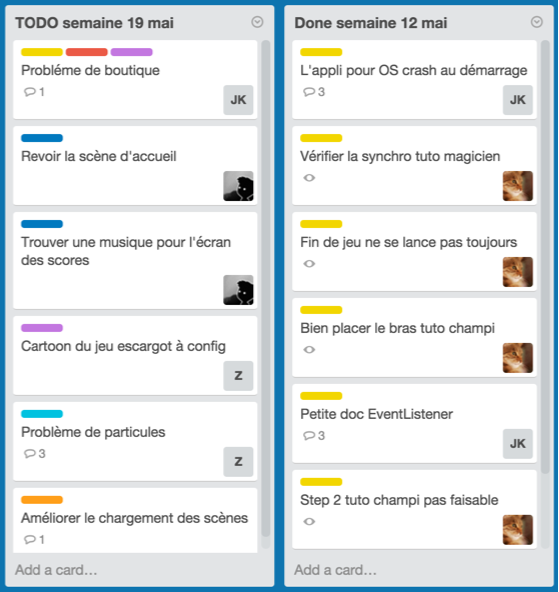
\includegraphics[scale=1]{./img/trello.png}}
\begin{center}
\textit{Exemple de colonnes en fin de projet}
\end{center}

\paragraph{}
Trello a aussi été utilisé comme mémo et pour archiver les ressources graphiques et sonores.

\paragraph{}
\noindent
\makebox[\textwidth]{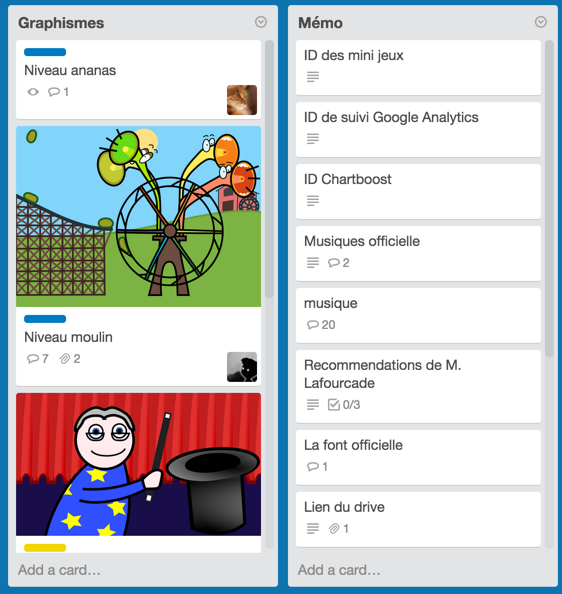
\includegraphics[scale=1]{./img/trello_autres.png}}
\begin{center}
\textit{Utilisation de Trello comme mémo et archives }
\end{center}

\paragraph{}
Cette méthode de travail avec Trello nous a permit d’être efficace 100\% du temps au travers de l’Internet. Il n’y avait jamais de temps mort et nous étions toujours clair dans notre direction tant que quelqu’un (chef de projet) s’occupait de crééer des tâches et de les organiser.

\subsection{Réunions}

\paragraph{}
Même si \textit{Trello} nous permet de travailler de façon indépendante, nous nous réunions très régulièremement pour travailler ensemble et fixer les nouveaux objectifs, de une à deux fois par semaines.

\paragraph{}
Pendant les longues séances de travail en collaboration (de 9h à 18h par exemple), nous utilisons un véritable tableau blanc pour noter les tâches en cours et les affecations. Exemples de tâches :

\begin{itemize}
\item Réadapter la taille du logo pause sur android v4.1 en écran 16:10 ;
\item Couper les 150ms du début du son tic.wav ;
\item Revoir l’animation du bras gauche du champignon.
\end{itemize}

\paragraph{}
Les tâches étant à 80\% de ce type (courtes et rapides), l’organisation est très importante pour être efficace.

\paragraph{}
De nombreuses heures de réunion étaient dédiés à la recherche de concept ou de remise en question des objectifs. Par exemple abandonner le développement d’un mini jeu trop complexe, ou en inventer de plus simples.

\subsection{Cycles itératifs}

\paragraph{}
Dés le départ, un développement par cycles itératifs a été choisit. Bien adapté pour le développement d’un jeu vidéo et surtout à cause de notre contrainte principale : notre liberté sur les choix.

\paragraph{}
Les premières semaines ont été dédiés à la réalisation de prototypes et de tests en augmentant toujours la difficulés, dans l’objectif de produire un moteur de jeu de rythme fonctionnel qui correspond aux besoins définis dans le cahier des charges.

\begin{itemize}
\item \textbf{Prototype 1} - Réalisation d’un cube qui bat à un rythme constant (3 jours)
\item \textbf{Prototype 2} - Réalisation d’un prototype de test de réussite (2 jours)
\item \textbf{Prototype 3} - Création de la première version du moteur de rythme (6 jours)
\item \textbf{Prototype 4} - Réalisation d’un prototype d’animations, connectés au moteur de rythme (4 jours) \emph{-> Le moteur n’est pas assez précis et doit être revu}
\item \textbf{Prototype 5} - Deuxième version du moteur de rythme (3 jours)
\item \textbf{Prototype 6} - Nouvelle tentative de connexion à des animations (1 jour) \emph{-> Test OK. On s’aperçoit que nous avons besoin de quart de temps dans le modèle et qu’il faut recommencer une nouvelle fois sa conception}
\item \textbf{Prototype 7} - Troisième version du moteur de rythme (4 jours)
\item Etc.
\end{itemize}

\paragraph{}
\noindent
\makebox[\textwidth]{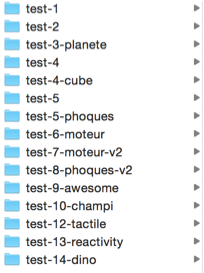
\includegraphics[scale=1]{./img/list-tests.png}}
\begin{center}
\textit{Les différents projets Unity de tests
}
\end{center}

\paragraph{}
A chaque nouveau test, un nouveau projet Unity. Au \textbf{test 14}, nous avons jugés que le moteur correspondait à nos attentez et nous avons ensuite itéré directement sur ce projet. C’est à ce moment (environs 1 mois après le début du projet) que le système de fonctionnement à changé et que nous avons fonctionné en micro-tâches.

\paragraph{}
Les dernières semaines ont été dédiés aux finitions sur le projet afin de rendre le jeu agréable avec un aspect “fini”.

\subsection{Github}

\paragraph{}
Un gestionnaire de version pour notre projet a bien sûr été utilisé et nous avons choisis le gestionnaire \emph{GitHub} qui offre de nombreux outils de statistiques très intéressants.

\paragraph{}
Déjà habitués à Git, nous l'avons utilisé pleinement et nous avons envoyés des \emph{commits} pour chaque modification fonctionelle. Nous sommes ainsi arrivé en fin de projet avec un cumule de de \textbf{900 commits}, globalement bien répartis entre nous quatre. (Avec plus de 2 millions de modifications dans les fichiers...).

\paragraph{}
\noindent
\makebox[\textwidth]{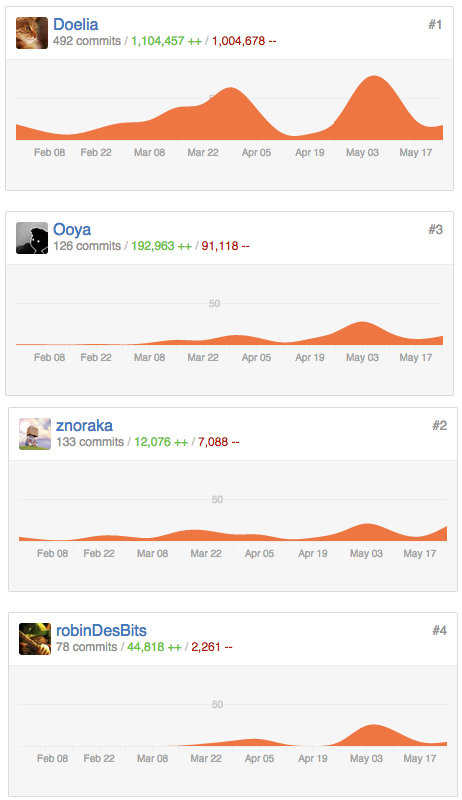
\includegraphics[scale=1]{./img/github_commits}}
\begin{center}
\textit{Réparition des commits dans le temps}
\end{center}

\paragraph{}
On remarque de nombreuses suppresions (presque autant que d’addition), prouvant l’évolution du projet et l’application des cycles itératifs. Le développement s’est fait continuellement dans le temps.

\subsubsection{Ponctualité hebdomadaire}

\noindent
\makebox[\textwidth]{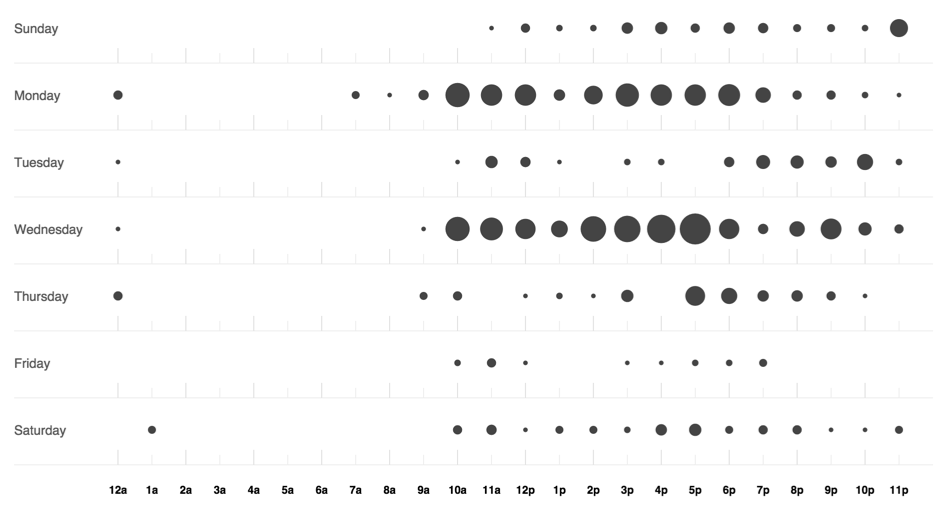
\includegraphics[scale=.7]{./img/punchcard.png}}
\begin{center}
\textit{Punchard de Github}
\end{center}

D’après les statistiques \emph{Github}, nous avons travaillé tous les jours de la semaine, avec une préférence pour le lundi et le mercredi en après midi et jusqu’en fin de soirée.

\subsubsection{Modélisation Gource}

Gource est une application qui permet de tracer en vidéo l’historique des commits qui construit l’architecture des fichiers d’un projet GIT.

\paragraph{}
Cette capture représente l’état final de l’architecture des fichiers du projet. La taille de la branche des tests démontre qu'ils ont effectivement constituée une grande partie du projet (Environs 30\%).

\paragraph{}
\noindent
\makebox[\textwidth]{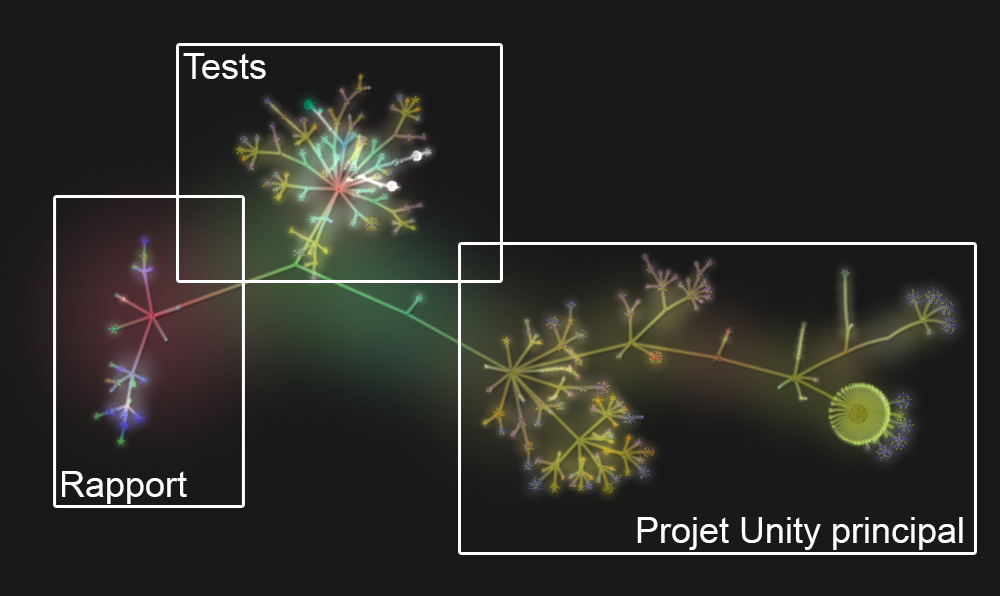
\includegraphics[scale=.4]{./img/gource_over.png}}
\begin{center}
\textit{Modélisation Gource en fin de projet}
\end{center}

\section{Résultat et comparaison avec le prévisionnel}

\paragraph{}
Globalement à 2 semaines avant la date finale, on peut juger que l'objectif a été atteint. 
Le jeu est jouable et tout est prêt pour qu'il soit mit en ligne sur l'Apple Store et le Play Store. Les tests auprès des utilisateurs ont été concluants.

\paragraph{}
La liste des \textit{couches} (prévues dans l'analyse) qui ont été développés sont les suivantes :
\begin{itemize}
\item 4 mini jeux pleinements fonctionnels ;
\item Des tutoriels pour chacun des mini jeux ;
\item Jeu jouable sur tout les téléphones sous Android et iOS ;
\item Système de débloquage des mini jeux et enregistrement du taux réussite ;
\item Monétisation avec de la publicité.
\end{itemize}

\paragraph{}
Les élements suivants n'ont pas été développés, par choix :
\begin{itemize}
\item Système de personnalisation ;
\item Mode de jeu infini répétitif ;
\item Editeur de niveau collaboratif.
\end{itemize}

\paragraph{}
Ces choix de retrait se sont fait suffisament tôt dans le projet (à mi-parcours pour être certain d'aboutire à un jeu fonctionnel. Nous avons préféré nous concentrer sur les tâches listées si dessus. Ce fut tout de même un travail important.

\paragraph{}
Nous sommes globalement satisfaits de notre gestion du temps, et nous pensons que notre organisation y a beaucoup contribué.
L'experience de créer un jeu de A à Z nous a beaucoup apprit et nous a permit de mettre en oeuvre beaucoup de concept sur la gestion de projets.



